\documentclass[tikz]{standalone}

% Font
\usepackage{mathpazo}
\usepackage{libertine}
\renewcommand*\sfdefault{phv}

\large

% Color
\usepackage{xcolor}
\definecolor{f1}{HTML}{F39019}
\definecolor{b1}{HTML}{DE6A10}
\definecolor{f2}{HTML}{51A7F9}
\definecolor{b2}{HTML}{0365C0}
\definecolor{f3}{HTML}{70BF41}
\definecolor{b3}{HTML}{00882B}

% tikz
\usepackage{tikz}
\tikzstyle{every node}=[font=\sffamily]
\usetikzlibrary{shapes,arrows,positioning,calc,decorations.markings,backgrounds}
\tikzstyle{c1} = [thick,draw=b1,fill=f1]
\tikzstyle{c2} = [thick,draw=b2,fill=f2]
\tikzstyle{c3} = [thick,draw=b3,fill=f3]
\tikzstyle{cg} = [thick,draw=gray!50,fill=gray!30]
\tikzstyle{rect} = [rectangle, minimum height=1cm]
\tikzstyle{roundrect} = [rect, rounded corners=.2cm]
\tikzstyle{io} = [trapezium, trapezium left angle=70, trapezium right angle=110]
\tikzstyle{arrow} = [thick,->,>=stealth]

\begin{document}
	
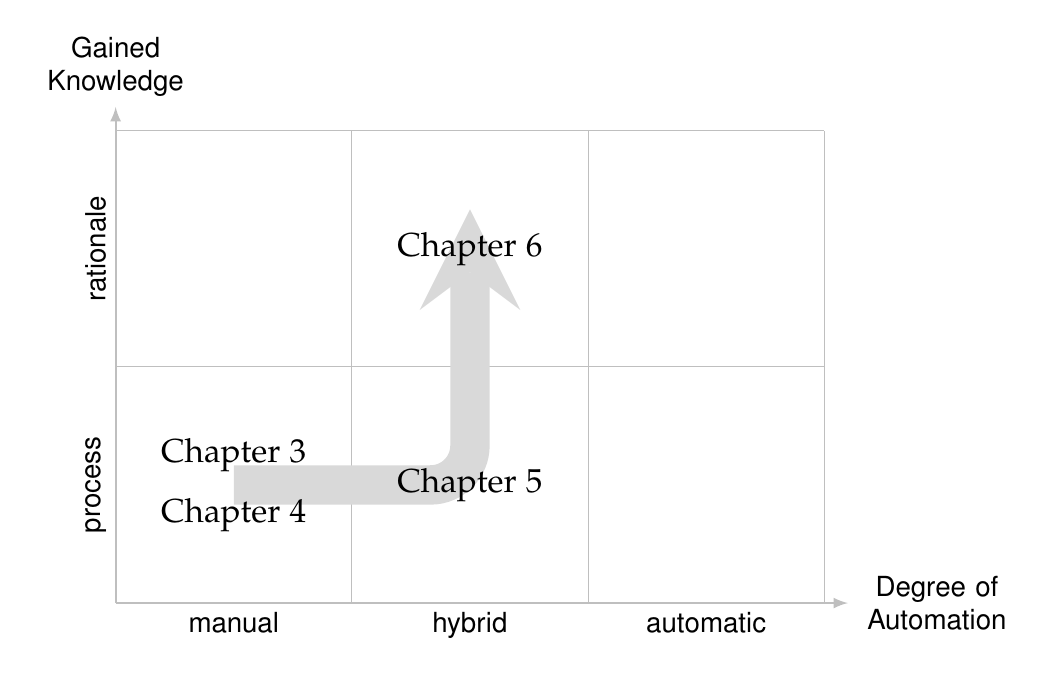
\begin{tikzpicture}
\draw [arrow,>=latex,draw=gray!50] (0,0) -- (9.3,0) node[right, text width=2cm, align=center] {Degree of Automation};
\draw [arrow,>=latex,draw=gray!50] (0,0) -- (0,6.3) node[above, text width=2cm, align=center] {Gained Knowledge};
\draw [draw=gray!50] (3,0) --++ (0,6) node {};
\draw [draw=gray!50] (6,0) --++ (0,6) node {};
\draw [draw=gray!50] (9,0) --++ (0,6) node {};
\draw [draw=gray!50] (0,3) --++ (9,0) node {};
\draw [draw=gray!50] (0,6) --++ (9,0) node {};

\node (manual) at (1.5,0) [below] {manual};
\node (hybrid) at (4.5,0) [below] {hybrid};
\node (auto) at (7.5,0) [below] {automatic};
\node (process) at (0,1.5) [above, rotate=90] {process};
\node (rationale) at (0,4.5) [above, rotate=90] {rationale};

\draw [arrow, draw=gray!30,line width=.5cm, rounded corners=.5cm] (1.5,1.5) -|(4.5,5);

\node at (1.5,1.5) [text width=3cm, align=center] {\large\rmfamily Chapter 3\\[.3cm]Chapter 4};
\node at (4.5,1.5) [text width=3cm, align=center] {\large\rmfamily Chapter 5};
\node at (4.5,4.5) [text width=3cm, align=center] {\large\rmfamily Chapter 6};

\end{tikzpicture}
	
\end{document}